\documentclass[11pt, a4paper, notitlepage, oneside]{article}
\usepackage[utf8]{inputenc}
\usepackage{url}
\usepackage{enumerate}
\usepackage{verbatim}
\usepackage{graphicx}
\usepackage{amsmath}
\usepackage{changepage}% http://ctan.org/pkg/changepage
\usepackage{lipsum}% http://ctan.org/pkg/lipsum
\graphicspath{ {images/} }

\usepackage[a4paper, total={6in, 8in}]{geometry}

%paragraph indentation
\setlength{\parindent}{4em} 

%paragraph spacing
\setlength{\parskip}{1em}

%Line spacing
% \renewcommand{\baselinestretch}{1.5}


\title{ \textbf{B. tech project: General Profit scheduling \\ report } }

\author{ Supervisor - Prof. Amit Kumar \\
Devansh Dalal (2012CS10224)  }

\begin{document}

\maketitle

\abstract{  The  following general scheduling problem is considered :  The  input consists  of n jobs,  each  with an release zero time, arbitrary size, and a monotone function specifying the cost incurred when the job is completed at a particular time(or the function can specify the profit gained if job is completed at a particular time). The objective is to find a schedule of minimum aggregate cost(or maximum total profit). 


This problem formulation is general enough to include many natural scheduling objectives such as weighted flow, weighted tardiness, and sum of flow squared etc. 


For this problem, most of the work has been done basically for special versions of function and with single processor. The problem is NP-hard even for 1 processor case\cite{janiak2007single}.
I will discuss the solution for 2 special cases of the problem in this report.The first result is based on the paper\cite{janiak2007single} which gives the a pseudo polynomial time algorithm dynamic programming formulation for single machines case  which is easily extended to multiple machines case using similar ideas. This case can also be modified to handles the preemption if necessary. While the second paper is a special case of the result from of the paper "The geometry of scheduling" \cite{bansal2010geometry} using their GSP to R2C reduction for zero release times. It gives a randomized polynomial-time algorithm for a single machine case with an O(1)-approximation ratio.

\section{Introduction}

We are given input which consists  of n jobs of arbitrary size, each with zero release times, m machines  and a non-increasing function specifying the profit gained when the job is completed by a particular time. The objective is to find a schedule of maximum aggregate profit.

\begin{figure}[!h]
\caption{Example of a Profit function for jobs}
\centering
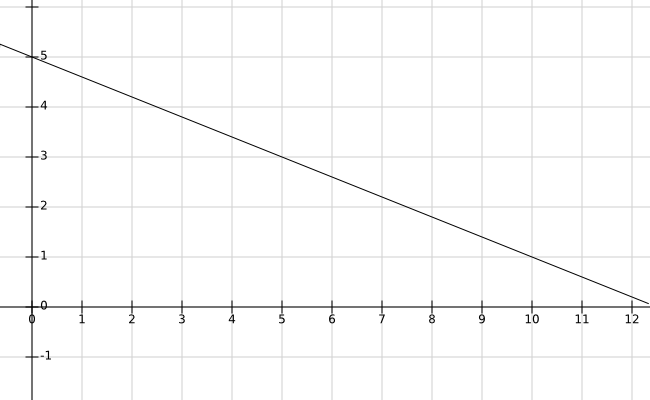
\includegraphics[width=0.5\textwidth]{save}
\end{figure}

When these profit functions $ g_i(t) $ are linearly decreasing, then there is polynomial time greedy solution for single machine case for the problem which given as follows:

\begin{enumerate}
\item Let T = sum of all the jobs.
\item schedule the jobs on the decreasing order of the value of 
$ g_i(0) - g_i(T)/p_i $ 
\end{enumerate}


\begin{figure}
\caption{Example of a Profit function for jobs}
\centering
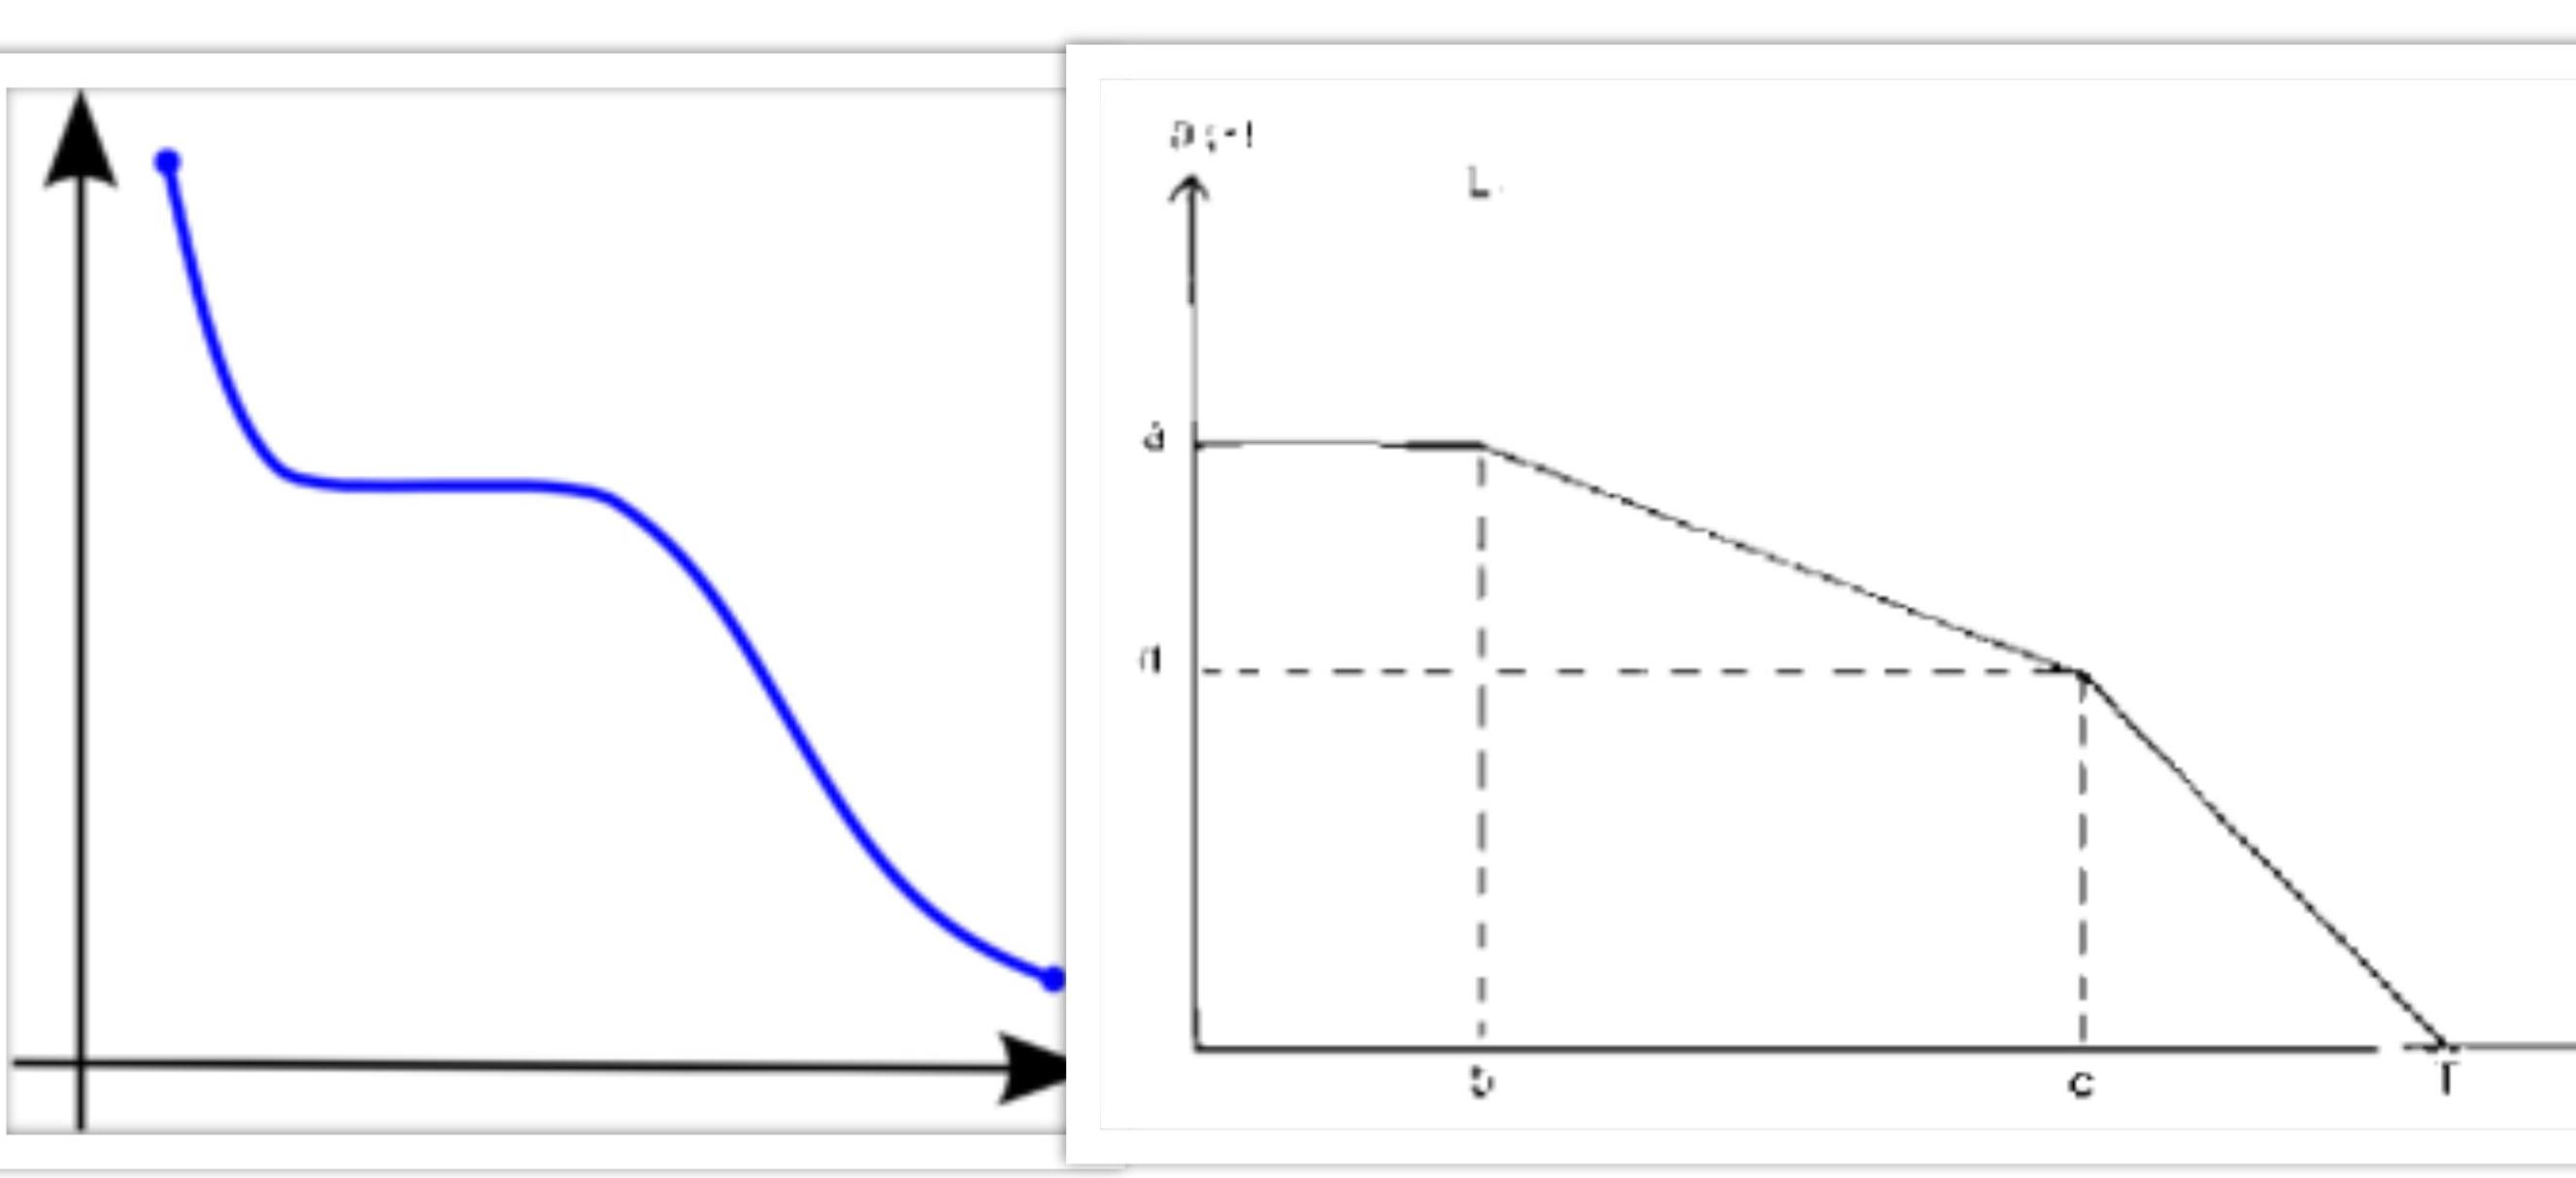
\includegraphics[width=0.5\textwidth]{dec}
\end{figure}


%%%%--------------------------------------------------------------------------------------------------------------------------------------------


















\section{Dynamic programming formulation for multiple machines}

In this special case the decreasing profit functions are first approximated as step-wise non-increasing functions before processing and then a pseudo polynomial time solution is constructed using DP with these functions.


\begin{figure}[!h]
\caption{Example of step-wise non-increasing profit functions}
\centering
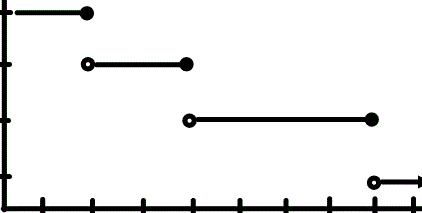
\includegraphics[width=0.5\textwidth]{step}
\end{figure}

so we assume the profit functions now have a form of type

$$
    w_i(C_i) = 
            \begin{cases} 
              w_{i1} & 0<C_i \leq d_{i1} \\
              w_{i2} & d_{i2}<C_i \leq d_{i3} \\
              : \\
              w_{i2} & d_{i k-1} < C_i  \\ 
            \end{cases}
$$

Suppose there are k time points at which the value of these function changes. Jobs will be considered in their natural order. We have k*m disjunctive sets of jobs:

$$
   X_1^1, X_2^1, ... , X_k^1, X_1^2, X_2^2, ... , X_k^2, .  , X_1^m, X_2^m, ... , X_k^m  
$$

\begin{figure}[!h]
\caption{Approximation of general function to step-wise non-increasing functions  }
\centering
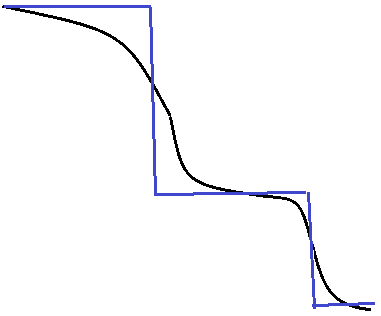
\includegraphics[width=0.5\textwidth]{func}
\end{figure}

where the jobs from the set $ X_1^2, X_2^2, ... , X_k^2 $ are scheduled on the machine $M_i$ in such a way that jobs from the set $X_q^i$ are sequenced before jobs from the set $X_q^{i+1}$ and processing of jobs from $X_q^i$ finishes before $d_q$, q = 1,...,k, and $d_k=inf $ .
Moreover, inside the set $X_q^i$ jobs are processed according to the non-decreasing order of $p_l^i$(processing time).Actually it does not matter in which order they are processed, but for the time being assume that they are processed using \textit{SPT}(shortest processing time first) algorithm. In the algorithm jobs will be assigned to the sets , which are empty at the beginning. We assume that assignment of the job $J^j$ to the set $X_q^i$ contributes $w_{jq}$ to the objective function.

Let us define a function
$$
    W_j(P_1^1, P_2^1, ... , P_k^1, P_1^2, P_2^2, ... , P_k^2, .  , P_1^m, P_2^m, ... , P_k^m)
$$ 
as the maximum possible profits for the partial schedule of first j jobs, for which sum of processing times of jobs assigned to the set $X_q^i$ is $P_q^i$

Thus, for j = 1,...,n we can calculate recurrently for all possible values of q = 1,...,k-1 and i = 1,...,m and obtain the optimal value of the objective function as

Initialization is given by
$$
    W_j(P_1^1)= 
            \begin{cases} 
              0 & if (j,P_1^1,...,P_1^1)=(0,...,0) \\
              -\infty & o.w \\
            \end{cases}
$$


$$
    W^* = \max_{q \in [1,k) |
    r \in [1,k-1) |
    i \in [1,m] } {W_n(P_1^1,...,P_{k-1}^m) ]}
$$


% \begin{figure}[!h]
% \caption{Optimal value of Profit functions for n jobs on m machines}
% \centering
% 
\includegraphics[width=0.5\textwidth]{formula}
% \end{figure}

The complete solution can be constructed by backtracking over the DP memoization table for the optimal solution. This formulation is quite flexible in the sense that it can be applied to more general cases. for example

\begin{enumerate}
    \item The jobs can have different processing times on different machines.
    \item Similarly profit functions can be different for same jobs on different machines.
    \item The solution can be extended to a more general case where the the release date of jobs is not zero.
    \item The solution can be optimized further by introducing other constraints to aviod computing the solution for bad states.
\end{enumerate}



% \newpage


\begin{figure}[!h]
\caption{complete recursion formula for m machines }
\centering
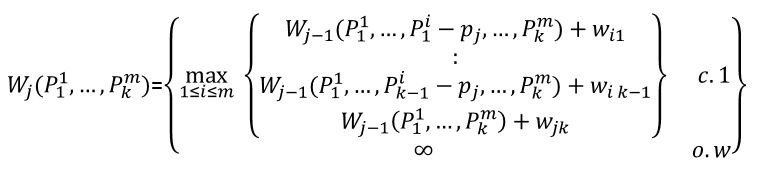
\includegraphics[width=0.5\textwidth]{last}
\end{figure}

















%%%%--------------------------------------------------------------------------------------------------------------------------------------------

    
    
    
    
    
    
    
    
    
    
    
    
    
    
    
    
    
    
\section{By reduction to geometric cover problem \cite{bansal2010geometry} }

\subsection{Notation and definitions}

\textit{General Scheduling Problem(GSP)}:The input consists of a collection of n jobs, and for each job j, a positive integer release time $r_j$, a positive integer size $ p_j $, and a cost or weight function $w_j(t) \geq 0 $ are given and the job can be scheduled at any each $ t_j \geq r_j $. And if a job is completed by time t, then a cost of $  \sum_{s=r_j+1}^{t} w_j(s)  $ is incurred and the goal is to minimize the total cost , $ \sum_{j=1}^n \sum_{s=r_j+1}^{C_j} w_j(t)  $, where $ C_j $ is the completion time of job j. 

\textit{Geometric set cover problem(R2C)}:The input consists of a collection $P$ of points in 2 dimensional space, and for each point $ p \in P $ and associated positive integer demand $d_p$. Each point $p \in P $ is specified by its coordinates $(x_p,y_p)$. Further input consists a collection $R$ of axis parallel rectangles, each of them abutting about y-axis. That is each rectangle $r \in R$ has the form $ (0,x_r)x(y_r^1,y_r^2)  $. In addition each rectangle $r \in R$ has an associated positive integer capacity $c_r$  and a positive integer weight $w_r$. The goal is to find a minimum weighted subset of rectangles such that for each point p , the total capacity of rectangles covering p is at least $d_p$. i.e. $\sum_{r \in R: p \in P}c_r \geq d_p$

% % % % % jobs, and forsssss each job j a positive integer release time $r_j$, a positive integer size $ p_j $, and a cost or weight function $w_j(t) \geq 0 $ for each $ t_j \geq r_j $. And if a job is completed by time t, then a cost of $  \sum_{s=r_j+1}^{t} w_j(s)  $ is incurred and the goal is to minimize the total cost , $ \sum_{j=1}^n \sum_{s=r_j+1}^{C_j} w_j(t)  $, where $ C_j $ is the completion time of job j.

Instead of dealing with profit functions for each jobs let's consider the problem in terms of the cost functions. 

\subsection{Reduction from GSP to R2C}
Here we are going to give the reduction from GSP to R2C problem which increases the value of the objective solution by at most a factor of 4 and does not decreases the optimal solution at the same time.

\textbf{lemma 1: } A polynomial-time $\alpha$-approximation algorithm for R2C implies a polynomial-time $4\alpha$ approximation algorithm for GSP 

\textit{Proof:} Let us assume we are given an arbitrary instance $ I $ of GSP, we create an instance $I'$ of R2C. Let us say a time $ t > r_j $ is of class $ k \geq 1 $ w.r.t job j if the cost of finishing j at time t lies in $ [2^{k-1},2^k-1] $ . i.e. $ \sum_{t'=1}^t w_j(t')  \in [ 2^{k-1},2^k-1 ] $ and similarly t is of class 0 if cost of finishing j is 0. 

Let $I_j^k$ denote the time intervals of time of class k w.r.t job j. Let T denote the the set of all endpoints of such intervals . Now for every pair of point $t_1,t_2 \in T $ consider the interval $ X= [t_1,t_2) $ where $t_1<t_2$ we create a point p in $ I' $ with demand $d_p=max(0, P(X)-|X| ) where P(X)$ denotes the total size of jobs released during interval X. Then for each job j and k>=0, we create a rectangle $ R_k^j = [0,r_j] x I_k^j  $ in I' with capacity $p_j$ and weight $2^k - 1 $. Note that all the rectangles corresponding to a single job are disjoint.

% \begin{figure}[!h]
% \caption{Example of covering a point with a rectangle}
% \centering
% 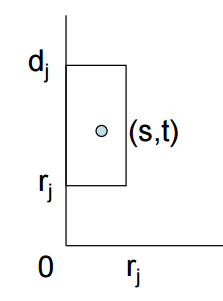
\includegraphics[width=0.5\textwidth,scale=0.1]{specialcase}
% \end{figure}

\begin{figure}
    \centerline{%
        \resizebox{0.6\textwidth}{!}{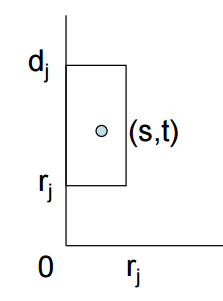
\includegraphics{specialcase}}%
    }
\end{figure}

\begin{figure}[!h]
\caption{Problem setting showing y-axis abutting rectangles covering points}
\centering
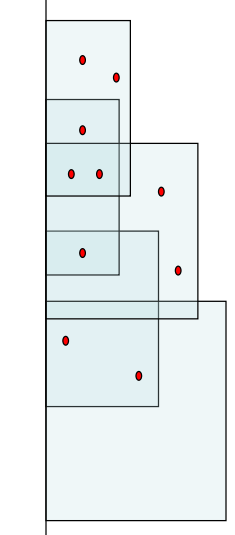
\includegraphics[width=0.5\textwidth]{r2c}
\end{figure}


\textbf{Lemma 2:} If there is a feasible solution S to I with objective value v, then there there is a feasible solution S' to I' with objective value at most 4v.
\textit{Proof:} For job j in I, let k(j) denote the class during which j finishes in S (i.e. k(j) is the smallest integer such that the cost incurred by j in S is  $ \leq 2^{k(j)} - 1)$ . Consider the solution S' obtained by choosing for each job j, the intervals . Clearly, each job contributes at most $ \sum_{i=0}^{k(j)} 2^i - 1 \leq 2(2^(k(j)) - 1) \leq  4x2^{k(j)}-1 $ , i.e. at most 4 times its contribution to S, and hence the total cost of S' is at most 4 times the cost of S.

It remains to show that S' is feasible, i.e. for any point p, the total capacity of rectangles covering p is at least $d_p$. Suppose p corresponds to the time interval X = [t1,t2) from I. Let $J_X$ denote the jobs that arrive during X. For each job $j \in J_X$ that completes after t2, there is exactly one rectangle $R_k^j$ that covers p. Since S is a feasible schedule, the total size of jobs in $J_X$ that can complete during X itself cannot be more than |X| = t2 - t1. Thus the jobs in JX that do not complete during X must have a total size of at least P(JX) - |X|, which is the covering requirement for p.

Similarly it can be proved that the cost of optimal solution is as large as the reduced problem using hall's theorem.

\subsection{With identical release times}

    WLOG, let $r_j=0$ for all jobs a=j =. In this case, The above reduction becomes simpler . In particular, the first dimension corresponding to release time becomes irrelevant and we obtain the one dimensional version of the geometric cover problem. i.e. All relevant intervals X are of form [0,t) and for each such interval we introduce a point (0,t) having demand D-t , where D is total size of all the jobs and we also introduce an interval corresponding to class k times with respect to each job j that has capacity $p_j$ and weight $2^k-1$.

This becomes a special case of the following Generalized Caching Problem.
Generalized Caching Problem: The input consists of a set of demands d(t) at various time steps t = 1,...,n. In addition there is a collection of time intervals I, where each interval I has weight $w_I$, size $c_I$ and span $[s_I,t_I]$ with $s_I,t_I \in  {1,... ,n}$. The goal is to find a minimum weight subset of intervals that covers the demand. That is, find the minimum weight subset of intervals S such that

$$
    \sum_{I \in S: t \in [S_I,t_I] } c_I \geq d_t \	for \  all \ t \in {1,...,n}.
$$

A 4-approximation of this problem was given by Bar-Noy et al \cite{bar2001unified} based on local ration technique. Their algorithm can equivalently be viewed as a primal dual algorithm applied to a linear program with knapsack cover inequalities [6]. This immediately implies a 16-approximation for GSP in the case of identical release times. \cite{bar2005equivalence}.



\section{Further Work}


\begin{enumerate}
    \item Still no good results known for the multiple machine case.
    \item Approximation for GSP to R2C problem can be improved.
    \item Can use better solution of the generalized caching problem.

\end{enumerate}



% \newpage
\medskip

\bibliographystyle{unsrt}%Used BibTeX style is unsrt
\bibliography{sample}

\end{document}
